\section{Análisis de resultados}%
\label{sec:analisisResultado}

Para realizar los análisis propuestos en en la figura \ref{fig:planpruebas}, se inicio considerando que sea posible observar

\begin{figure}[H]
	\centering
	\begin{subfigure}[b]{0.495\linewidth}
		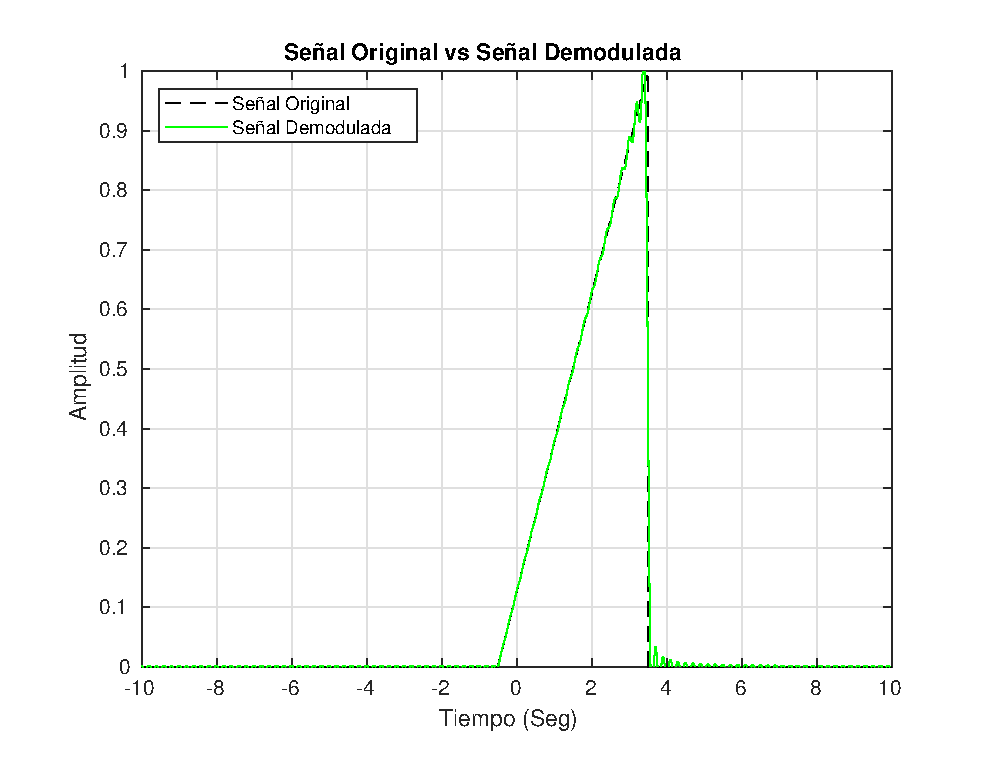
\includegraphics[width=5.1cm]{img/Comp_Tim/Comp_Tim.eps}
		\caption{\scriptsize Error de fase de 60 grados.}
		\label{subfig:inoutTiempo}
	\end{subfigure}
	\begin{subfigure}[b]{0.495\linewidth}
		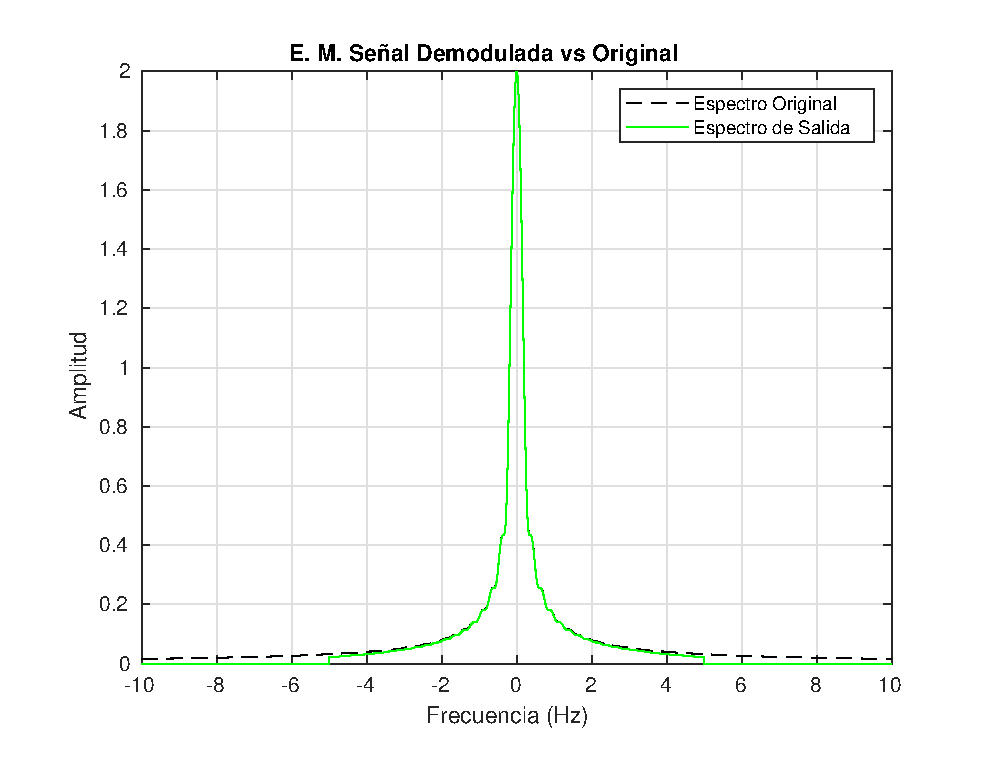
\includegraphics[width=5.1cm]{img/Comp_EM/Comp_EM.eps}
		\caption{\scriptsize Sin error de fase.}
		\label{subfig:inoutFrecuencia0}
	\end{subfigure}
	\vspace{-3mm}
	\caption{\scriptsize Señales de salida con errores de sincronismo en fase.}
	\label{fig:inoutSistema}
	\vspace{-5mm}
\end{figure}

\subsection{Desarrollo del objetivo clave 1-Análisis de resultados sin introducir errores de sincronismo}

\subsection{Desarrollo del objetivo clave 2-Introducir errores de sincronismo en fase}

Para el escenario planteado de falta de sincronismo de fase, se realizaron iteraciones de la simulación variando el valor de sincronismo de fase en pasos de 45 grados.
Se hace uso de los valores de Energía y MSE para tener una aproximación cuantitativa de la modificación que sufre la señal de salida con respecto a la señal de entrada.

\begin{figure}[H]
	\centering
	\begin{subfigure}[b]{0.49\linewidth}
		\def\svgwidth{5cm}
		\input{img/DFase0/DFase0.pdf_tex}
		\caption{\scriptsize Sin error de fase.}
		\label{subfig:DFase0}
	\end{subfigure}
	\begin{subfigure}[b]{0.49\linewidth}
		\def\svgwidth{5cm}
		\input{img/DFase60/DFase60.pdf_tex}
		\caption{\scriptsize Error de fase de 60 grados.}
		\label{subfig:DFase60}
	\end{subfigure}
	\begin{subfigure}[b]{0.49\linewidth}
		\def\svgwidth{5cm}
		\input{img/DFase90/DFase90.pdf_tex}
		\caption{\scriptsize Error de fase de 90 grados.}
		\label{subfig:DFase90}
	\end{subfigure}
	\begin{subfigure}[b]{0.49\linewidth}
		\def\svgwidth{5cm}
		\input{img/DFase180/DFase180.pdf_tex}
		\caption{\scriptsize Error de fase de 180 grados.}
		\label{subfig:DFase180}
	\end{subfigure}
	\vspace{-3mm}
	\caption{\scriptsize Señales de salida con errores de sincronismo en fase.}
	\label{fig:graficasfase}
	\vspace{-5mm}
\end{figure}

Es evidente que el sincronismo de fase introduce atenuación lineal en el rango de 0 a 90 grados (figuras \ref{subfig:DFase0}, \ref{subfig:DFase60}, \ref{subfig:DFase90}). Sin embargo, es interesante apreciar que, en el siguiente rango de frecuencias, esta atenuación se revierte con el signo contrario. Por lo que la MSE alcanza su valor máximo de error en 180 grados (figura \ref{fig:erroresFase}), que es cuando la señal es mas similar a la señal de entrada, pero multiplicada por -1 (figura \ref{subfig:DFase180}).
\begin{table}[H]
	\centering
	\caption{\scriptsize}
	\label{tab:varacionFrecuencia}
	\vspace{-3mm}
	\tiny\begin{tabular}{|l|c|c|c|c|c|}
		\hline
		Variación Fase         & 0       & 45      & 90      & 135            & 180   \\ \hline
		MSE Input-Output       & 0.00064  & 0.02940 & 0.33310    & 0.96830    & 1.32860 \\ \hline
		Energía Salida $A_c=2$ & 1.32800 & 0.66  & 0.0001 & 0.66360           & 1.32860 \\ \hline
		Energía Entrada        & 1.3332  & 1.3332  & 1.3332  & 1.3332         & 1.3332 \\ \hline \hline
		Variación Fase   & 180     & 225     & 270     & 315      & 360   \\ \hline
		MSE Input-Output       & 1.32860 & 0.96870 & 0.33350 & 0.02950   & 0.00064 \\ \hline
		Energía Salida $A_c=2$ & 1.32860 & 0.66440 & 0.00001 & 0.66360   & 1.32800 \\ \hline
		Energía Entrada        & 1.3332  & 1.3332  & 1.3332  & 1.3332   & 1.3332 \\ \hline
	\end{tabular}

\end{table}

% \begin{table}[H]
% 	\centering
% 	\caption{\scriptsize}
% 	\label{tab:variacionFrecuencia2}
% 	\vspace{-3mm}
% 	\tiny\begin{tabular}{|l|c|c|c|}
% 		\hline
% 		{Variación Frecuencia} & {MSE Input-Output} & {Energía Salida $A_c=2$} & {Energía Entrada} \\ \hline
% 		{-10}                  & 0.3988             & 0.3265                   & 1.332             \\ \hline
% 		{-1}                   & 0.50210            & 0.6629                   & 1.332             \\ \hline
% 		{-0.5}                 & 0.65               & 0.6603                   & 1.332             \\ \hline
% 		{-0.1}                 & 0.40410            & 0.2493                   & 1.332             \\ \hline
% 		{-0.01}                & 0.00076            & 1.2924                   & 1.332             \\ \hline
% 		{0}                    & 0.00064            & 1.328                    & 1.332             \\ \hline
% 		{0.01}                 & 0.00074            & 1.2927                   & 1.332             \\ \hline
% 		{0.1}                  & 0.40370            & 0.2486                   & 1.332             \\ \hline
% 		{0.5}                  & 0.65770            & 0.6604                   & 1.332             \\ \hline
% 		{1}                    & 0.50210            & 0.6629                   & 1.332             \\ \hline
% 		{10}                   & 0.39880            & 0.3265                   & 1.332             \\ \hline
% 	\end{tabular}
% \end{table}

Los valores máximos de energía se tienen en 0 y 180 grados, sin embargo, en estos mismos puntos se tienen los valores mínimo y máximo de energía de la señal. Esto nos permite concluir que la energía por si sola, no es un referente ideal para medir la integridad o la perdida de información de una señal que ha atravesado un sistema.
\begin{figure}[H]
	\centering
	\def\svgwidth{8.8cm}
	\tiny\input{img/ErroresFase/ErroresFase.pdf_tex}
	\caption{\scriptsize Variación de fase contra MSE y energía.}
	\vspace{-3mm}
	\label{fig:erroresFase}
\end{figure}
Al ser la señal evaluada una señal no periódica con espectro de frecuencia infinito centrado en banda base, cualquier filtrado pasa bajo introduce distorsión lineal, sin embargo, si no se tiene en cuenta la distorsión generada por el filtro, se puede afirmar que la modificación de la señal producida por el de-sincronismo de fase no califica como distorsión lineal ya que aparentemente afecta a todas las componentes de frecuencia dentro del rango del modulador de una manera similar.

\subsection{Desarrollo del objetivo clave 3-Introducir errores de sincronismo en frecuencia}
Para este escenario se realizaron iteraciones de la simulación variando el valor de sincronismo en frecuencia para los valores observados en la tabla. Se realizó de esta manera ya que a diferencia de como ocurría en los errores de fase, en los errores de frecuencia no se observa una relación lineal de ocurrencia y pequeños cambios en el sincronismo afectan de manera significativa a la señal, sobre todo, en valores cercanos a una variación de frecuencia igual a cero.
% \begin{table}[H]
% 	\centering
% 	\caption{\scriptsize }
% 	\label{tab:varacionFrecuencia}
% 	\vspace{-3mm}
% 	\tiny\begin{tabular}{|l|c|c|c|c|c|}
% 		\hline
% 		Variación Frecuencia   & -10     & -1      & -0.5    & -0.1    & -0.01   \\ \hline
% 		MSE Input-Output       & 0.3988  & 0.50210 & 0.65    & 0.40410 & 0.00076 \\ \hline
% 		Energía Salida $A_c=2$ & 0.3265  & 0.66290 & 0.66030 & 0.24930 & 1.29240 \\ \hline
% 		Energía Entrada        & 1.3332  & 1.3332  & 1.3332  & 1.3332  & 1.3332  \\ \hline \hline
% 		Variación Frecuencia   & 0.01    & 0.1     & 0.5     & 1       & 10      \\ \hline
% 		MSE Input-Output       & 0.00074 & 0.40370 & 0.65770 & 0.50210 & 0.39880 \\ \hline
% 		Energía Salida $A_c=2$ & 1.29270 & 0.24860 & 0.66040 & 0.66290 & 0.32650 \\ \hline
% 		Energía Entrada        & 1.3332  & 1.3332  & 1.3332  & 1.3332  & 1.3332  \\ \hline
% 	\end{tabular}
% 
% \end{table}

\begin{table}[H]
	\centering
	\caption{\scriptsize}
	\label{tab:variacionFrecuencia2}
	\vspace{-3mm}
	\tiny\begin{tabular}{|l|c|c|c|}
		\hline
		{Variación Frecuencia} & {MSE Input-Output} & {Energía Salida $A_c=2$} & {Energía Entrada} \\ \hline
		{-10}                  & 0.3988             & 0.3265                   & 1.332             \\ \hline
		{-1}                   & 0.50210            & 0.6629                   & 1.332             \\ \hline
		{-0.5}                 & 0.65               & 0.6603                   & 1.332             \\ \hline
		{-0.1}                 & 0.40410            & 0.2493                   & 1.332             \\ \hline
		{-0.01}                & 0.00076            & 1.2924                   & 1.332             \\ \hline
		{0}                    & 0.00064            & 1.328                    & 1.332             \\ \hline
		{0.01}                 & 0.00074            & 1.2927                   & 1.332             \\ \hline
		{0.1}                  & 0.40370            & 0.2486                   & 1.332             \\ \hline
		{0.5}                  & 0.65770            & 0.6604                   & 1.332             \\ \hline
		{1}                    & 0.50210            & 0.6629                   & 1.332             \\ \hline
		{10}                   & 0.39880            & 0.3265                   & 1.332             \\ \hline
	\end{tabular}
\end{table}

Es posible apreciar que para los valores cercanos a la frecuencia central (en este caso banda base), la distorsión y la energía sirven como indicadores de integridad de la señal. Siendo esto apreciable en la figura \ref{subfig:DFreq0} y \ref{subfig:DFreq001}.

\begin{figure}[H]
	\centering
	\begin{subfigure}[b]{0.49\linewidth}
		\def\svgwidth{5cm}
		\input{img/DFreq0/DFreq0.pdf_tex}
		\caption{\scriptsize En sincronismo.}
		\label{subfig:DFreq0}
	\end{subfigure}
	\begin{subfigure}[b]{0.49\linewidth}
		\def\svgwidth{5cm}
		\input{img/DFreq001/DFreq001.pdf_tex}
		\caption{\scriptsize Error de 0.01 Hz.}
		\label{subfig:DFreq001}
	\end{subfigure}
	\begin{subfigure}[b]{0.49\linewidth}
		\def\svgwidth{5cm}
		\input{img/DFreq01/DFreq01.pdf_tex}
		\caption{\scriptsize Error de 0.1 Hz.}
		\label{subfig:DFreq01}
	\end{subfigure}
	\begin{subfigure}[b]{0.49\linewidth}
		\def\svgwidth{5cm}
		\input{img/DFreq1/DFreq1.pdf_tex}
		\caption{\scriptsize Error de 1 Hz.}
		\label{subfig:DFreq1}
	\end{subfigure}
	\vspace{-3mm}
	\caption{\scriptsize Señales de salida con errores de sincronismo en frecuencia.}
	\label{fig:graficasfreq}
	\vspace{-5mm}
\end{figure}

En valores de cambio de frecuencia superiores a los mencionados, la señal es reemplazada por un trozo de onda senoidal de frecuencia directamente proporcional al de-sincronismo en frecuencia aplicado. La señal original aparece como envolvente de esta onda. Este comportamiento se presenta hasta que el de-sincronismo es mayor al ancho de banda del filtro pasa bajo. Esto debido a que la componente de frecuencia de la señal original deformada por la falta de sincronismo en frecuencia es absorbida por este filtro.
\begin{figure}[H]
	\centering
	\def\svgwidth{8.8cm}
	\tiny\input{img/ErroresFrecuencia/ErroresFrecuencia.pdf_tex}
	\caption{\scriptsize Variación de frecuencia contra MSE y energía.}
	\vspace{-3mm}
	\label{fig:erroresFreucencia}
\end{figure}
Esta tendencia se observa en la figura \ref{fig:erroresFreucencia}, donde se aprecia que en los extremos, la energía cae, y el error medio cuadrático comienza a estabilizarse a valores cercanos a 0.33, los cuales se dan cuando la señal no está presente (tal como se aprecia en el caso de desfase a 90 grados).


\subsection{Desarrollo del objetivo clave 4-Introducir ambos tipos de errores de sincronismo.}


\begin{figure}[H]
	\centering
	\begin{subfigure}[b]{0.49\linewidth}
		\def\svgwidth{5cm}
		\input{img/EMF90_freq0/EMF90_freq0.pdf_tex}
		\caption{\scriptsize En sincronismo.}
		\label{subfig:EMF90_freq0}
	\end{subfigure}
	\begin{subfigure}[b]{0.49\linewidth}
		\def\svgwidth{5cm}
		\input{img/EMF90_freq001/EMF90_freq001.pdf_tex}
		\caption{\scriptsize Error de 0.01 Hz.}
		\label{subfig:EMF90_freq001}
	\end{subfigure}
	\begin{subfigure}[b]{0.49\linewidth}
		\def\svgwidth{5cm}
		\input{img/EMF90_freq01/EMF90_freq01.pdf_tex}
		\caption{\scriptsize Error de 0.1 Hz.}
		\label{subfig:EMF90_freq01}
	\end{subfigure}
	\begin{subfigure}[b]{0.49\linewidth}
		\def\svgwidth{5cm}
		\input{img/EMF90_freq1/EMF90_freq1.pdf_tex}
		\caption{\scriptsize Error de 1 Hz.}
		\label{subfig:EMF90_freq1}
	\end{subfigure}
	\vspace{-3mm}
	\caption{\scriptsize Señales de salida con errores de sincronismo en fase de $90^\circ$ y variación en frecuencia.}
	\label{fig:graficasFase90freq}
	\vspace{-5mm}
\end{figure}
